\section{Systematic Uncertainties}
\label{sec:Systematics}

This section describes a number of sources of systematic uncertainties
that are relevant for the presented  analysis. To account for differences in the observed and simulated 
detector response a set of corrections is applied at the level of object reconstruction  
and at event level as described in chapter~\ref{chap:obj}. 
The uncertainties due to such corrections are referred to as detector-related systematic 
uncertainties and are addressed in section~\ref{sec:sys:sys_det}. 
For all processes whose contributions are predicted from simulation, also theory-related
systematic uncertainties need to be accounted for. These include uncertainties on the cross-section and
 on the acceptance of events after the given analysis selection criteria and 
are  described in section~\ref{sec:sys_theory}$\,.$
Further systematic uncertainties related to the background measurements with dedicated control data 
are described in Sections~\ref{sec:embsys} and~\ref{sec:qcdsys}$\,.$

Each source of systematic uncertainty can contribute separately to the uncertainty on the
final event yield and on the shape of the $\mmc$
distribution which is used as final discriminating variable in the statistical interpretation of data. Systematic uncertainties
that affect the shape of the mass distribution are
documented in appendix~\ref{appendix:shapeNPs}. Uncertainty on the \mmc shape distribution 
are found to be negligible for all except the embedded sample, for which significant 
deviation from the nominal distribution are found in the b-vetoed category only. 
Systematic uncertainties that do not affect the
shape of the mass distribution and have an impact on the event yield of less than 0.5\% for each process are 
neglected.
%hey in fact do not have any significant effect on the final expected limits.


\subsection{Detector-related Systematics Uncertainties}
\label{sec:sys:sys_det}
Systematic uncertainties related to object reconstruction and event-by-event 
corrections are based on the calibration measurements of the relevant parameter. Each 
of those parameters correspond to a nuisance parameter in the probability model used for the  statistical interpretation
as described in Section~\ref{sec:result}.
Each parameter is varied independently by one standard deviation  according to its measured
uncertainty. The corresponding impact on the  yield of simulated events is evaluated for each signal and background sample.
In the following, detector-related uncertainty are  described in more details.
Tables~\ref{tab:ExpSys:btag} and~\ref{tab:ExpSys:bveto} briefly summarize the impact of these uncertainties on the 
predicted sample yields. 


\paragraph{Luminosity}
The integrated luminosity of the 8 TeV data recorded with the ATLAS detector during 2012 is measured 
to be $20.3 ~ fb^{-1}$ \cite{luminosity} with an uncertainty  of  2.8\%.

\paragraph{Pileup}
Simulated events are re-weighted to reproduce the average number of interactions per bunch crossing $<\mu>$ as seen in data. 
Those event weights have an uncertainty which is propagated to each simulated sample.
%It has been seen
%that a proper description of the minimum bias vertex multiplicity is obtained if the $<\mu>$ 
%value in MC is first scaled by a factor of $1.11 \pm 0.03$ before re-weighting to match data. The uncertainty
%on this value is taken as a systematic uncertainty for the analysis.

\paragraph{Trigger Efficiency}
is corrected in simulation to match (on the average) the one observed in data. Those correction weights 
are evaluated as a function of $\pt$ and $\eta$ of the corresponding leptons and have associated uncertainties. 
Systematic uncertainties on both the single electron and electron-muon trigger efficiency are taken into account 
independently and range approximately from 1-2\%.

In the embedded $\Ztt$ sample, the trigger is emulated by applying weights  according to  the event
topology. Those weights are related to the ones described above
and have similar uncertainties. Trigger efficiency uncertainty for the embedded sample 
 are considered uncorrelated with those of other samples.

\paragraph{Electrons}
Two sources of uncertainty on reconstructed electron objects are considered:
the first  related to electron identification and reconstruction efficiencies ("Electron ID"), 
the second  related to electron energy scale and resolution corrections.
The energy scale uncertainties are described by a set of six different nuisance parameters~\cite{eleEnergy}.
However, only a few of them give a non-negligible contribution to the analysis. Two of them are found
to affect the shape of the \mmc distribution and are considered independently: uncertainty
arising from the electron  momentum measurement with $Z \rightarrow ee$ data ("Electron Zee") 
and the one related to low momentum electrons ("Electron LOWPT"). 
All other uncertainties related to energy scale and resolution are summed in quadrature ("Electron E").

\paragraph{Muons}
The uncertainty on muon identification efficiency depends on the charge and momentum of the muon.
Typically these uncertainties are of the order of a fraction of percent, and are referred as "Muon ID". 
The uncertainties on the muon energy scale and resolution are considered independently for the inner detector 
and muon spectrometer measurements and are hen  added in quadrature to estimate the final uncertainty ("Muon E").

\paragraph{Taus-Jets}
The jets from the hadronically decaying $\tau$ leptons are only considered 
in the analysis by applying a veto on their presence in an event. Uncertainties on both $\tau$-jet energy scale 
and identification efficiency have been investigated and are found to be negligible for this analysis.

\paragraph{Jets}
The systematic uncertainties on the Jet Energy Scale (JES) are described by multiple sets of nuisance parameters~\cite{JES}
related to different effects and jet energy components, for example the sensitivity to pileup effects or
to the flavour composition of the jet. The overall uncertainty on the JES ranges 
between 3\% and 7\%, depending on the $\pt$ and $\eta$ of the jet. 
The overall impact of the JES uncertainty on the analysis yields is shown in Tables~\ref{tab:ExpSys:btag} and~\ref{tab:ExpSys:bveto}
by summing all component in quadrature, while in the statistical interpretation of data
those uncertainties are considered uncorrelated.
Systematic uncertainty due to the jet resolution ("Jet Resolution") are obtained by smearing the jet energy 
according to the measured  uncertainty which ranges from 10-20\% depending on the direction of the jet.
%The recommendation \cite{TWIKI_JETMET} to propagate each individual 
% source of uncertainty through the full analysis is followed. In this analysis the reduced set of fourteen uncertainties, know as 
% \verb=InsituJES2012_14NP=, have been considered: these include two uncertainties for eta inter calibration, four pile-up 
% uncertainties, a high-$\pt$ uncertainty and an uncertainty for MC non-closure. Of these, only the terms "JES Effective 1", 
% "JES Effective 2" and "JES Effective 3", the pileup uncertainty as a function of the number of primary vertices ("JES Pileup-NPV") and the uncertainty due to the jet area ("JES Pileup-Rho") have a significant effect on the event yields. Additionally, 
% the uncertainty related to the fraction of quark to gluon jets ("JES Flav. Comp") and on the different response to them ("JES Flav. Resp.") are considered. The additional uncertainty assigned to the b-jet energy scale, referred as "JES B", is also 
% significant to this analysis. Uncertainties related to theory and modelling ("JES EtaModelling") also contribute to this 
% analysis. Finally the effect of the jet energy resolution ("JES Resolution") is evaluated applying a smearing to the jets, the 
% resulting effect on the yield is symmetrised.

\paragraph{b-Tagging}  Corrections are applied to simulation
to match the b-tagging efficiency observed  in data. Uncertainties on the knowledge 
of the b-tagging efficiencies for the 70\% $\epsilon_b^{\ttbar}$ working point of the MV1 b-tagger are
considered~\cite{BtaggingScaleFactors,BtaggingScaleFactorsNew}. These uncertainties range from 5-10\% in dependence on the $\pt$ of the jet. 
The effect of those uncertainties is evaluated independently for the
 b-quark, c-quark and light or gluon initiated jets and referred to respectively 
 as "B  Eff", "C Eff" and "L Eff". The tagging and mis-tagging efficiency uncertainties 
 are considered to be fully anti-correlated. 

\paragraph{Missing Transverse Energy}
The effect of the energy scale uncertainties for all  physics objects is propagated to the \met calculation.
In addition, uncertainty on the energy scale and resolution due to the remaining unassociated 
calorimeter energy deposits, the ``soft-terms'', is considered and estimated to be of the order of 10\%~\cite{ETMISS}. 
\met uncertainties are independently propagated through the analysis and are
added in quadrature, this final term is referred to as the "MET" uncertainty.


%\paragraph{Summary} A summary of the effect of the experimental and theoretical systematic uncertainties on signal and background yields for the b-tag and b-veto channels are shown in Table~\ref{tab:ExpSys:btag} and Table~\ref{tab:ExpSys:bveto}, respectively. It should 
%be noted that the gluon fusion  signal sample suffers of poor statistics in the b-tag category. 
%Hence, some of the yield differences reported are statistically dominated for these samples.
%%	As a solution the mean value between all the sample mass point can be taken as measure of the single systematic, 
%However the gluon fusion production mode has a negligible contribution in b-tag category.
\begin{table}[!htp]
  \centering
  \begin{tabular}{lccccc}
    \hline\hline
      	      		   \multicolumn{6}{c}{ b-vetoed event category,  Uncertainties on event yields (\%)}  \\
     \hline
      Source             & Signal bbH & Signal ggH & \Ztautau &  Top 	& Other	 \\
    \hline
Electron ID  		 &2.4		   &2.3		     &2.9 (\bf{s})	     &1.4	&1.6	 \\
Electron E.	  	 &0.4		   &0.5		     &0.4	     &0.5	&0.9	 \\
Electron LOWPT	  	 &0.3		   &0.5		     &0.4 (\bf{s})	     &0.0	&1.2  \\ 
Electron Zee	  	 &0.4		   &0.4		     &0.4 (\bf{s})	     &0.1	&0.3	 \\
Muon ID 		 &0.3		   &0.3		     &0.3	     &0.3	&0.3	 \\
Muon E.		  	 &0.1		   &0.1		     &0.1	     &0.5	&0.5	 \\
Trigger Single	Ele.  	 &0.6		   &0.6		     &0.5	     &0.9	&0.9	 \\
Trigger Dilep.	  	 &1.0		   &1.0		     &1.3	     &0.2	&0.3	 \\
Embedding MFS	  	 &-		   &-		     &0.1 (\bf{s})   &-		&-	 \\
Embedding Iso.	  	 &-		   &-		     &0.0 (\bf{s})   &-		&-	 \\
JES		  	 &0.6		   &0.7		     &-		     &1.0	&1.2	 \\
JER		  	 &0.5		   &0.3		     &-		     &0.6	&0.3	 \\
B Eff		  	 &1.8		   &0.0		     &-		     &12.0	&0.8	 \\
C Eff	  		 &0.0		   &0.1		     &-		     &0.1	&0.0	 \\
L Eff	  		 &0.0		   &0.1		     &-		     &0.2 	&0.1	 \\
Pileup			 &0.5		   &0.8		     &0.4	     &0.3	&0.3	 \\
MET  		  	 &0.2		   &0.8 	     &0.1	     &0.2	&0.5	 \\
%Acceptance		 &		   &		     &		     &		&	  \\
%Cross Section	  	 &-		   &-		     &5.0	     &5.5	&5.9	 \\
Luminosity	  	 &2.8 		   &2.8	 	     &2.8 	     &2.8 	&2.8 	 \\

    \hline
    \hline
  \end{tabular}
  \caption{Impact of the experimental systematic uncertainties on the event yields in different
	simulated samples in the b-vetoed event category. Here "Other" refers to the sum of all remaining background 
	samples: $\Wlnu$, 
	dibosons, $\Zll$ and single top quark processes. The signal produced in association with b-quarks  and via 
	gluon fusion is considered separately assuming $m_{A}=150$ GeV and $\tan\beta=20$. 
	Uncertainty that impacts the \mmc mass distribution are noted with the symbol (\textbf{s}).} 
 \label{tab:ExpSys:bveto}
\end{table}

	
\begin{table}[tp]
  \centering
  \begin{tabular}{lccccc}
    \hline\hline
      	      		   \multicolumn{6}{c}{ b-tagged event  category, Uncertainties on event yields (\%)}  \\
     \hline
      Source             & Signal bbH 	   & Signal ggH      & \Ztautau      &  Top 	& Other	 \\
    \hline
Electron ID  		 &2.3		   &2.6		     &	2.8          &1.8	&2.0	 \\
Electron E	  	 &0.7		   &1.2		     &0.5	     &0.5	&0.9	 \\
Electron LOWPT	  	 &0.4		   &0.0		     &0.4	     &0.1	&0.4	 \\ 
Electron Zee	  	 &0.3		   &0.6		     &0.4	     &0.6	&0.5	 \\
Muon ID 		 &0.3		   &0.3	   	     &0.3	     &0.3	&0.3	 \\
Muon E		  	 &0.5		   &0.8		     &0.1	     &0.1	&0.2	 \\
Trigger Single	Ele.  	 &0.7		   &0.5		     &0.5	     &0.8	&0.8	 \\
Trigger Dilepton  	 &1.0		   &1.2		     &1.4	     &0.6	&0.6	 \\
Embedding MFS	  	 &-		   &-		     &0.0	     &-		&-	 \\
Embedding Iso.	  	 &-		   &-		     &1.3	     &-		&-	 \\
JES		  	 &2.7		   &7.3		     &-		     &10.0	&7.0	 \\
JER		  	 &1.4		   &6.3		     &-		     &2.9	&3.0	 \\
B Eff		  	 &10.2		   &3.1		     &-		     &2.6	&5.0	 \\
C Eff		  	 &0.2		   &4.3		     &-		     &0.0	&1.2	 \\
L Eff		  	 &0.4		   &8.0		     &-		     &0.1	&1.2	 \\
Pileup			 &0.4		   &0.7		     &0.4	     &0.4	&0.9	 \\
MET 		  	 &0.7		   &0.5 	     &0.2	     &1.0	&1.2	 \\
%Acceptance		 &		   &		     &		     &		&	  \\
%Cross Section	  	 &-		   &-		     &5.0	     &5.5	&7.1	 \\
Luminosity	  	 &2.8 		   &2.8	 	     &2.8 	     &2.8 	&2.8 	 \\

    \hline
    \hline
  \end{tabular}
  \caption{Impact of the experimental systematic uncertainties on the event yields in different
	simulated samples in the b-taged event category. Here "Other" refers to the sum of all remaining background 
	samples: $\Wlnu$, 
	dibosons, $\Zll$ and single top quark processes. The signal produced in association with b-quarks  and via 
	gluon fusion is considered separately assuming $m_{A}=150$ GeV and $\tan\beta=20$.} 

  \label{tab:ExpSys:btag}
\end{table}




\subsection{Theoretical Uncertainties}
\label{sec:sys_theory}
%\subsection{Simulated Cross-Section Uncertainties}


\begin{table} [!t]
\centering
\begin{tabular}{c c c }
\hline
\hline
Generator & Process & Uncertainty \\ [0.5ex]
\hline
ALPGEN & $Z \rightarrow \tau\tau / ee /\mu\mu$ & $\pm 5\%$ \\
POWHEG & \ttbar					& $\pm 5.5\%$\\
ALPGEN & $W  \rightarrow \tau\nu / e\nu /\mu\nu$&  $\pm  5\%$ \\
AcerMC & single top & $\pm 13 \%$ \\
HERWIG & dibosons & $\pm 6 \%$ \\
SHERPA & $bbA$/$h$/$H$  ($m_{A} \ge 120$~GeV)     & $-(<20)$\%,  $+(<9)$ \%\\
SHERPA & $bbA$/$h$/$H$  ($m_{A} =   110$~GeV)     & $-(<25)$\%,  $+(<9)$ \%\\
SHERPA & $bbA$/$h$/$H$  ($m_{A} =   100$~GeV)     & $-(<28)$\%,  $+(<9)$ \%\\
SHERPA & $bbA$/$h$/$H$  ($m_{A} =    90$~GeV)     & $-(<30)$\%,  $+(<9)$ \%\\
POWHEG & $ggA$/$h$/$H$  ($m_{A} \le 300$~GeV)     & $<$ 15\%\\  [0.5ex]
\hline \hline 
\end{tabular}
\caption{Cross-section uncertainties for background and signal processes, $\tan\beta = 20$ is assumed for all signal samples.}
\label{table:sys_xsec}
\end{table}


Uncertainties on the cross-sections that have been used to normalize
the contribution of simulated samples to the integrated luminosity of analyzed data are reported in
Table~\ref{table:sys_xsec}. These
uncertainties include contributions due to parton distribution
functions (PDFs), the choice of the value of the strong coupling constant,
the renormalisation and factorisation scales.  Furthermore, the
uncertainties on the signal cross-section depend on the  $\tan\beta$ value, the nature of the 
Higgs boson ($A$/$h$/$H$) and its mass.

The impact  of systematic uncertainties due to various Monte Carlo tuning
parameters for the description of the  underlying event and
lepton kinematic properties is considered.
Since the distribution of the invariant mass of all visible $\tau$ lepton decay products is found to be not affected by these systematic,
uncertainties
% as an example see
%Figure~\ref{fig:theory_mass}, 
only the variation in the acceptance is considered as a systematic uncertainty.
The acceptance uncertainties for the simulated ALPGEN $\Ztautau$  sample, which is 
used for the normalization of the embedded sample, 
are estimated at the common selection stage to be 4\% \cite{2010SMLLSupportNote}.
%\footnote{A bit old result, to be reviewed. Depends also on the
%embedding choice}
Since additional selection criteria  are applied directly to the embedded sample, 
no further acceptance uncertainties are considered. Acceptance uncertainties on the yield of 
$t\bar{t}$ simulated events are estimated to be  2\%~\cite{ttbaremu}. %\textcolor{red}{still to be added}.
%evaluated
%\footnote{also here is not totally clear yet} 
%by the difference between MC@NLO and POWHEG in
%the data-driven background estimate. 
%For other, single and dibosons
%production as well as single top production a 2\% uncertainty is
%assumed.
The acceptance uncertainties on dibosons and single top quark production are estimated to be 2\%~\cite{2010SMLLSupportNote}.
%\footnote{preliminary, this is following LEP-Had note, we
%  should cite some previous result here.}.

Uncertainties on the signal acceptance have been estimated with signal 
samples produced  varying generator parameters. The impact on the selection
 of leptons, $\tau$-jet  and jets is evaluated at the particle level, prior to 
simulation of the detector response. This truth-level study is implemented within the Rivet framework
\cite{RIVET}, where the b-tagging is performed by identifying the b-quarks and applying
 weights according to the measured ATLAS b-tagging
efficiencies \cite{BtaggingScaleFactors}. The variation of the acceptance
with respect to the nominal Monte Carlo tune has  been considered as
a source of systematic uncertainty. For signal a total acceptance 
uncertainty varies from 4\% to 30\% depending on $\mA$, production process 
and on the analysis category.

%The acceptance uncertainties of the two signal production modes are
%evaluated separately because of the use of different generators for each. For
%b-quark associated production, generated with SHERPA,
%the CKKW matching parameter $Q_{cut}$ has been varied from its default
%of $\sqrt{20 ~ GeV/E_{CMS}}$ to values of $\sqrt{15 ~ GeV/E_{CMS}}$
%and $\sqrt{30 ~ GeV/E_{CMS}}$. The factorisation scale was varied up
%and down by a factor of two and the renormalisation scale by a factor of
%10\%. Uncertainties due to the PDFs were determined by taking the RMS
%of the acceptance of the 52 error sets of the CT10 PDF set.  These
%effects are summarized in Table~\ref{table:sys_bba}. For a total
%uncertainty, all effects are summed in quadrature giving a total
%uncertainties that varies from 4\% to 30\% depending on $\mA$ and on the
%analysis category.  For gluon fusion production, generated with POWHEG
%and Pythia 8, the initial and final state
%radiation uncertainties were varied up and down, and the
%renormalisation and factorisation scales were varied simultaneously
%(the renormalisation scale by 10\% and the factorisation scale by factor 2\%).
%PDFs uncertainties were handled in the same way as for the $b$-quark
%associated production.  These variations are summarized in Table
%\ref{table:sys_gga}.  The uncertainties shown in Tables
%\ref{table:sys_bba} and \ref{table:sys_gga} are based on samples with
%$m_{A} = 120 \text{ GeV}$.  Results for the mass points 90, 200
%and 300 GeV are shown in Appendix \ref{appendix:additional} of this note.
 


%\begin{table}[tdp]
%  \begin{center}
%   \label{table:sys_bba}
%   \begin{tabular}{lccccc}
%\hline \hline
% Event yields       & b-tag deviation [\%]  & b-veto deviation [\%] \\
%\hline
%CKKW down &    $ -3.1 \pm 0.9 $ &      $ 0.4 \pm 0.4 $ \\
%CKKW up &     $ -8.3 \pm 0.9 $ &      $ 2.9 \pm 0.4 $ \\
%Fac. scale down &    $ 15.5 \pm 1.0 $ &   $ -4.2 \pm 0.4 $ \\
%Fac. scale up &     $ -19.8 \pm 0.8 $ &    $ 5.6 \pm 0.4 $ \\
%Ren. scale down &      $ 0.4 \pm 0.9 $ &     $ -0.3 \pm 0.4 $ \\
%Ren. scale up &     $ 0.8 \pm 0.9 $ &      $ 0.5 \pm 0.4 $ \\
%PDF &     $\pm 0.1 $ 		& $\pm 0.2 $ \\
%\hline
%Total  (up) &     $ 13.5 \pm 1.6$ &                    $ 6.3 \pm 0.8$ \\
%Total  (down) &     $ -21.7 \pm 1.5$ &                    $ -4.2 \pm 0.6$ \\ 
%\hline \hline
%	\end{tabular}
%   \caption{Signal acceptances for several systematic deviations of the theory parameters contributing to the b-quark associated production of Higgs bosons. The different variations are added in quadrature to a total uncertainty on the signal acceptance in the b-tag and b-veto channels.}
%  \end{center}
%\end{table}
%
%
%\begin{table}[tdp]
%  \begin{center}
%   \label{table:sys_gga}
%    \begin{tabular}{lccccc}
 %   \hline \hline
% Event yields      &   b-tag deviation [\%] &   b-veto deviation [\%] \\
%\hline
%ISR up & $ 20.3 \pm 8.1 $ 		& $ -1.2 \pm 0.6 $ \\
%ISR down & $ 3.6 \pm 7.2 $ 		& $ 0.4 \pm 0.6 $ \\
%FSR up & $ 16.6 \pm 7.8 $ 		& $ -0.2 \pm 0.6 $ \\
%FSR down & $ -3.6 \pm 6.8 $	 	& $ -0.7 \pm 0.6 $ \\
%Ren./Fac. scales up & $ 9.4 \pm 7.5 $ 	& $ 0.0 \pm 0.6 $ \\
%Ren./Fac. scales down & $ 2.5 \pm 7.1 $ & $ -0.5 \pm 0.6$ \\
%PDF &     $\pm 0.0 $ &$\pm  0.1 $ \\
%\hline
%Total (up) &    $ 28.2 \pm 16.9 $ &     $ 0.4 \pm 0.6$ \\
%Total (down) &    $ -3.6 \pm 6.8 $ &     $ -1.5 \pm 1.2$ \\ 
%\hline \hline
%	\end{tabular}
%   \caption{Signal acceptances for several systematic deviations of the theory parameters contributing to the Higgs boson production through gluon fusion. The different variations are added in quadrature to a total uncertainty on the signal acceptance in the b-tag and b-veto channels.}
%  \end{center}
%\end{table}


%%%%%%%%%%%%%%%%%%%%%%%%%%Figure Lorentz%%%%%%%%%%%%%%%%%%%%%%
%\begin{figure}[tp]
%\begin{center}
%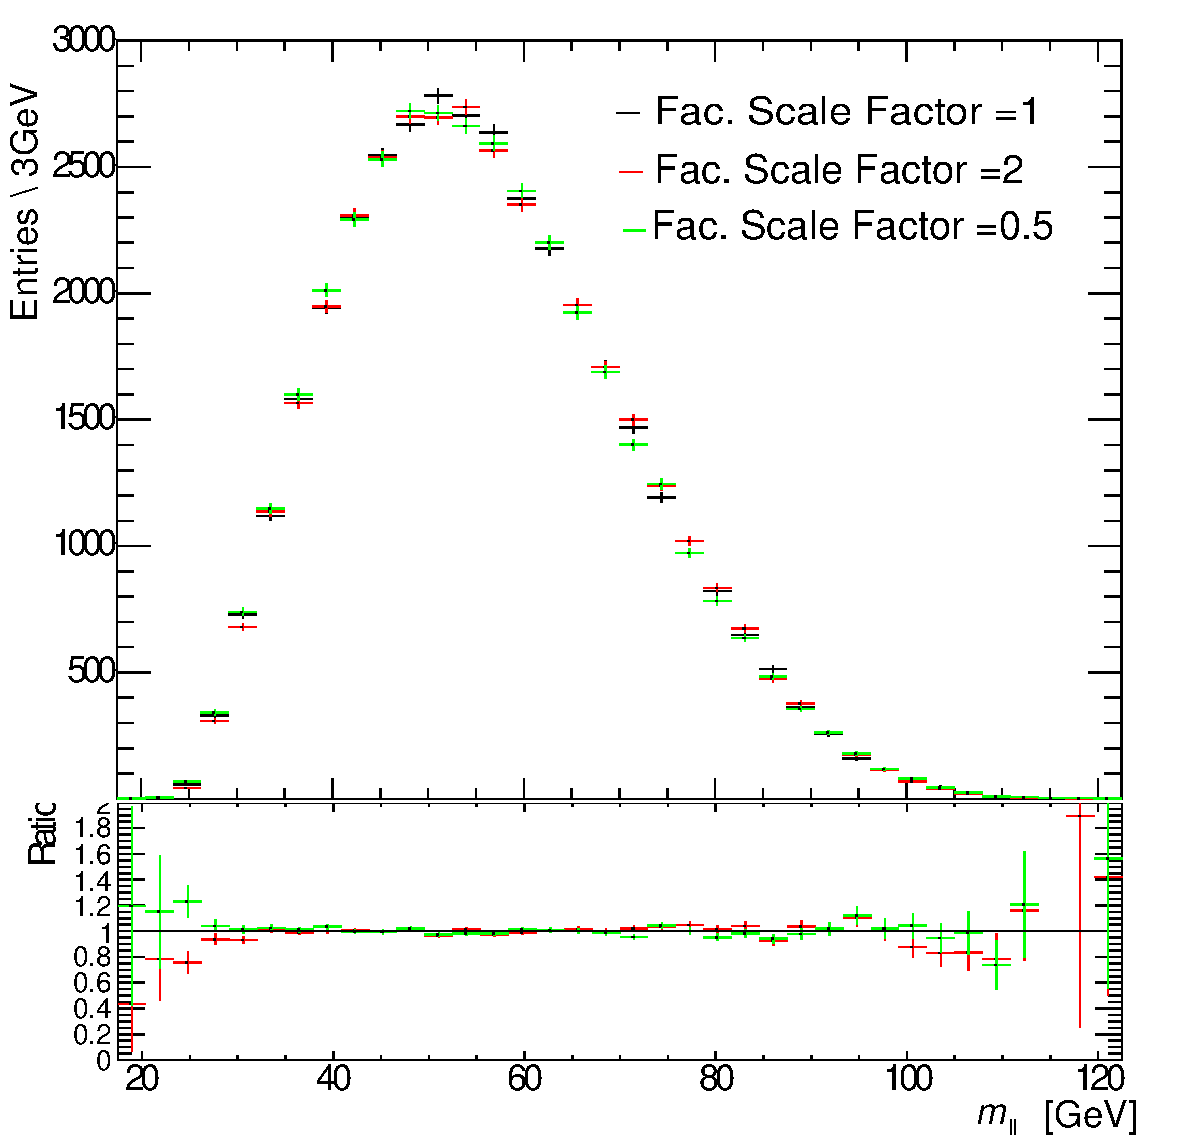
\includegraphics[width=0.65\textwidth]{figure/facs_mll_bveto2}
%\end{center}
%\caption{ Distribution of the invariant mass of all visible $\tau$-lepton decay products 
%for different choices of the factorisation scale. The shown distribution is 
%for gluon fusion produced signal in the b-vetoed event category.}
%\label{fig:theory_mass}
%\end{figure}
%


\subsection{Systematic Uncertainties of the \Ztautau Embedded Sample}\label{sec:embsys}

An important element of the embedding method is the subtraction of the 
calorimeter cells associated with the muons in the original \Zmumu event and their substitution with those from the simulated $\tau$ lepton
decays. To make a conservative estimate of the systematic uncertainty on this procedure, 
the energy of the subtracted cells is scaled up or down by 30\%. The analysis is repeated with those modified 
samples and the relative uncertainty is referred as "EMB\_MFS". This uncertainty affects mainly the shape of the \mmc mass 
distribution, shown in Figure~\ref{fig:EMBMFS}.


\begin{figure}[tp]
	\begin{center}
	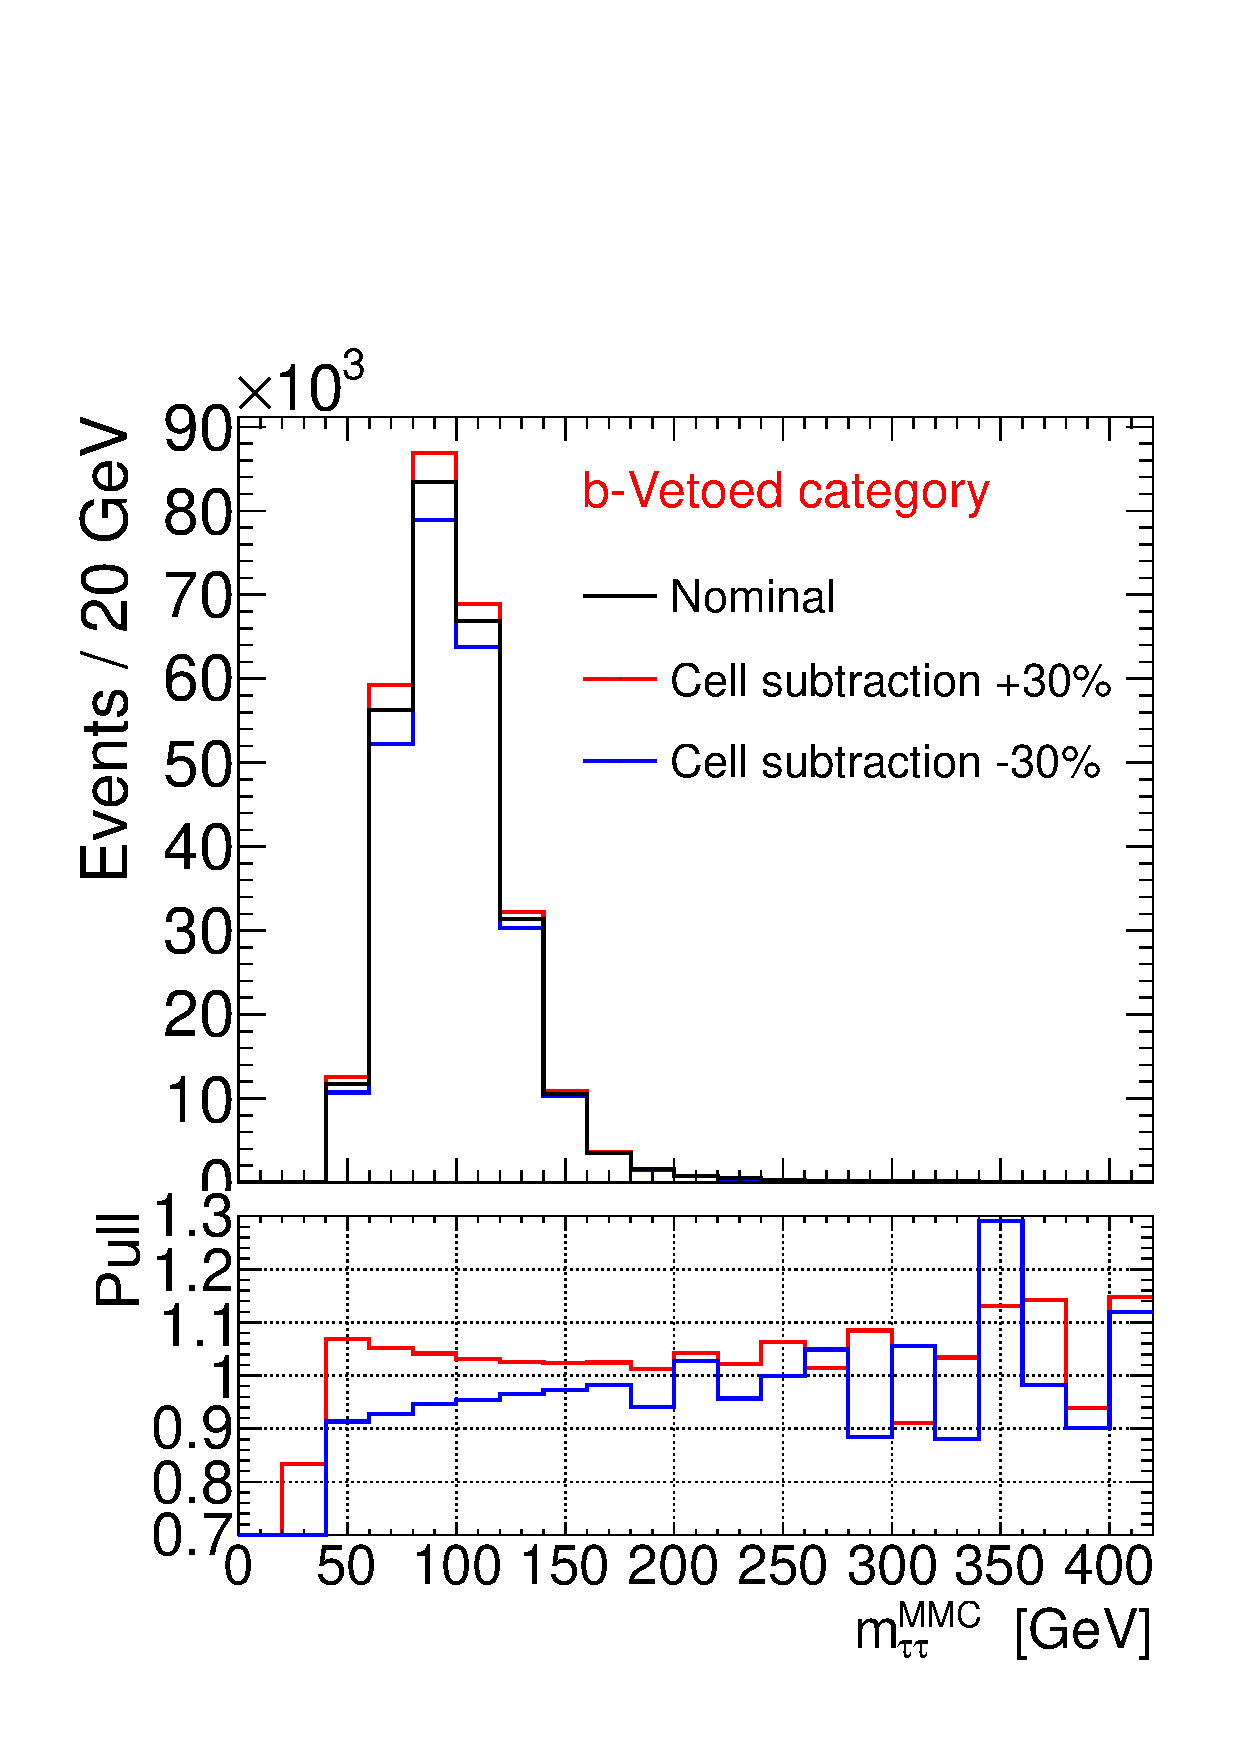
\includegraphics[width=0.49\textwidth]{figure/systematics/emb_sys_veto_MFS.pdf}
	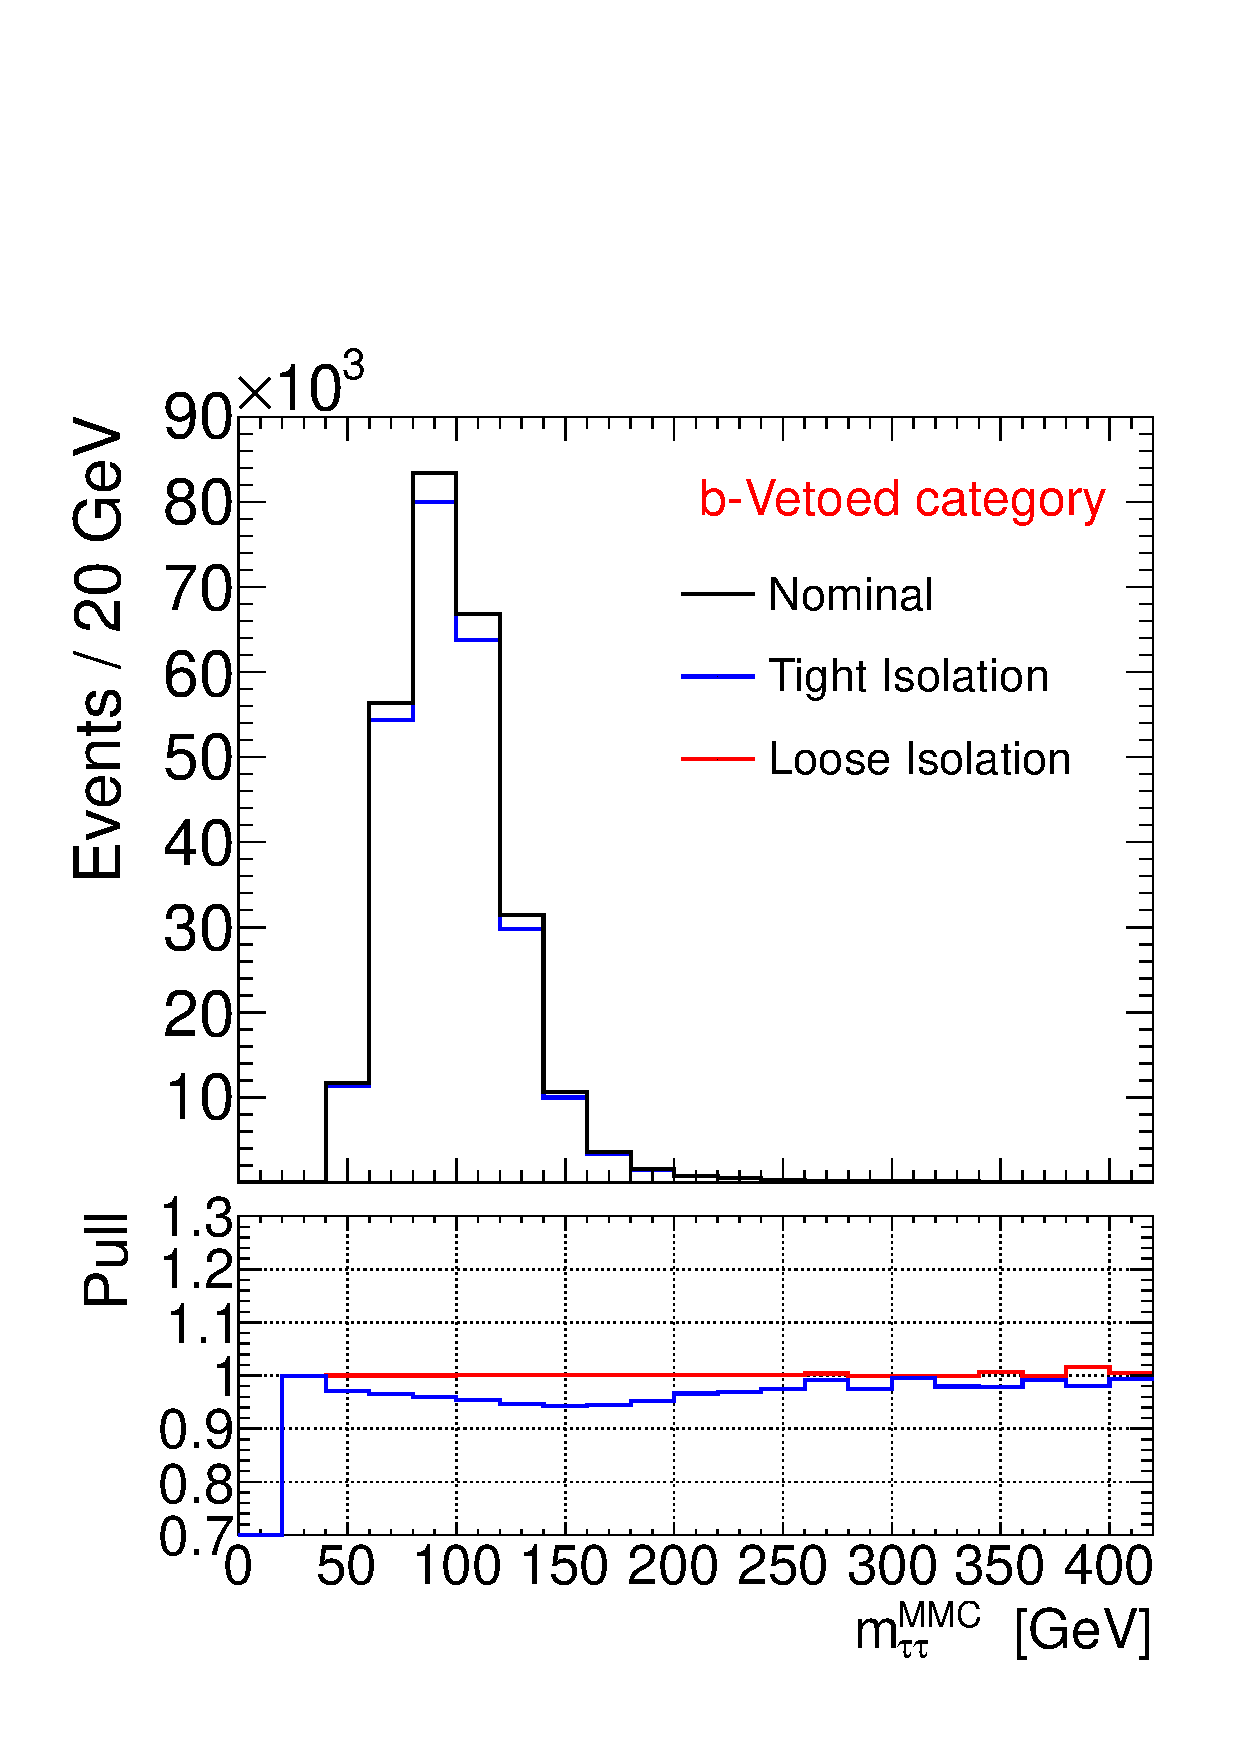
\includegraphics[width=0.49\textwidth]{figure/systematics/emb_sys_veto_iso.pdf}
	\end{center}
	\caption{Impact of EMB\_MFS (left) and EMB\_ISO (right) systematic uncertainties on the $\mmc$ mass distribution for in the  embedded sample.
	Significant impact is observed only in the b-vetoed event category.}
	\label{fig:EMBMFS}
\end{figure}

%\begin{figure}[htp]
%     \begin{center}
%
%        \subfigure[]{%
%            \label{fig:mvis}
%            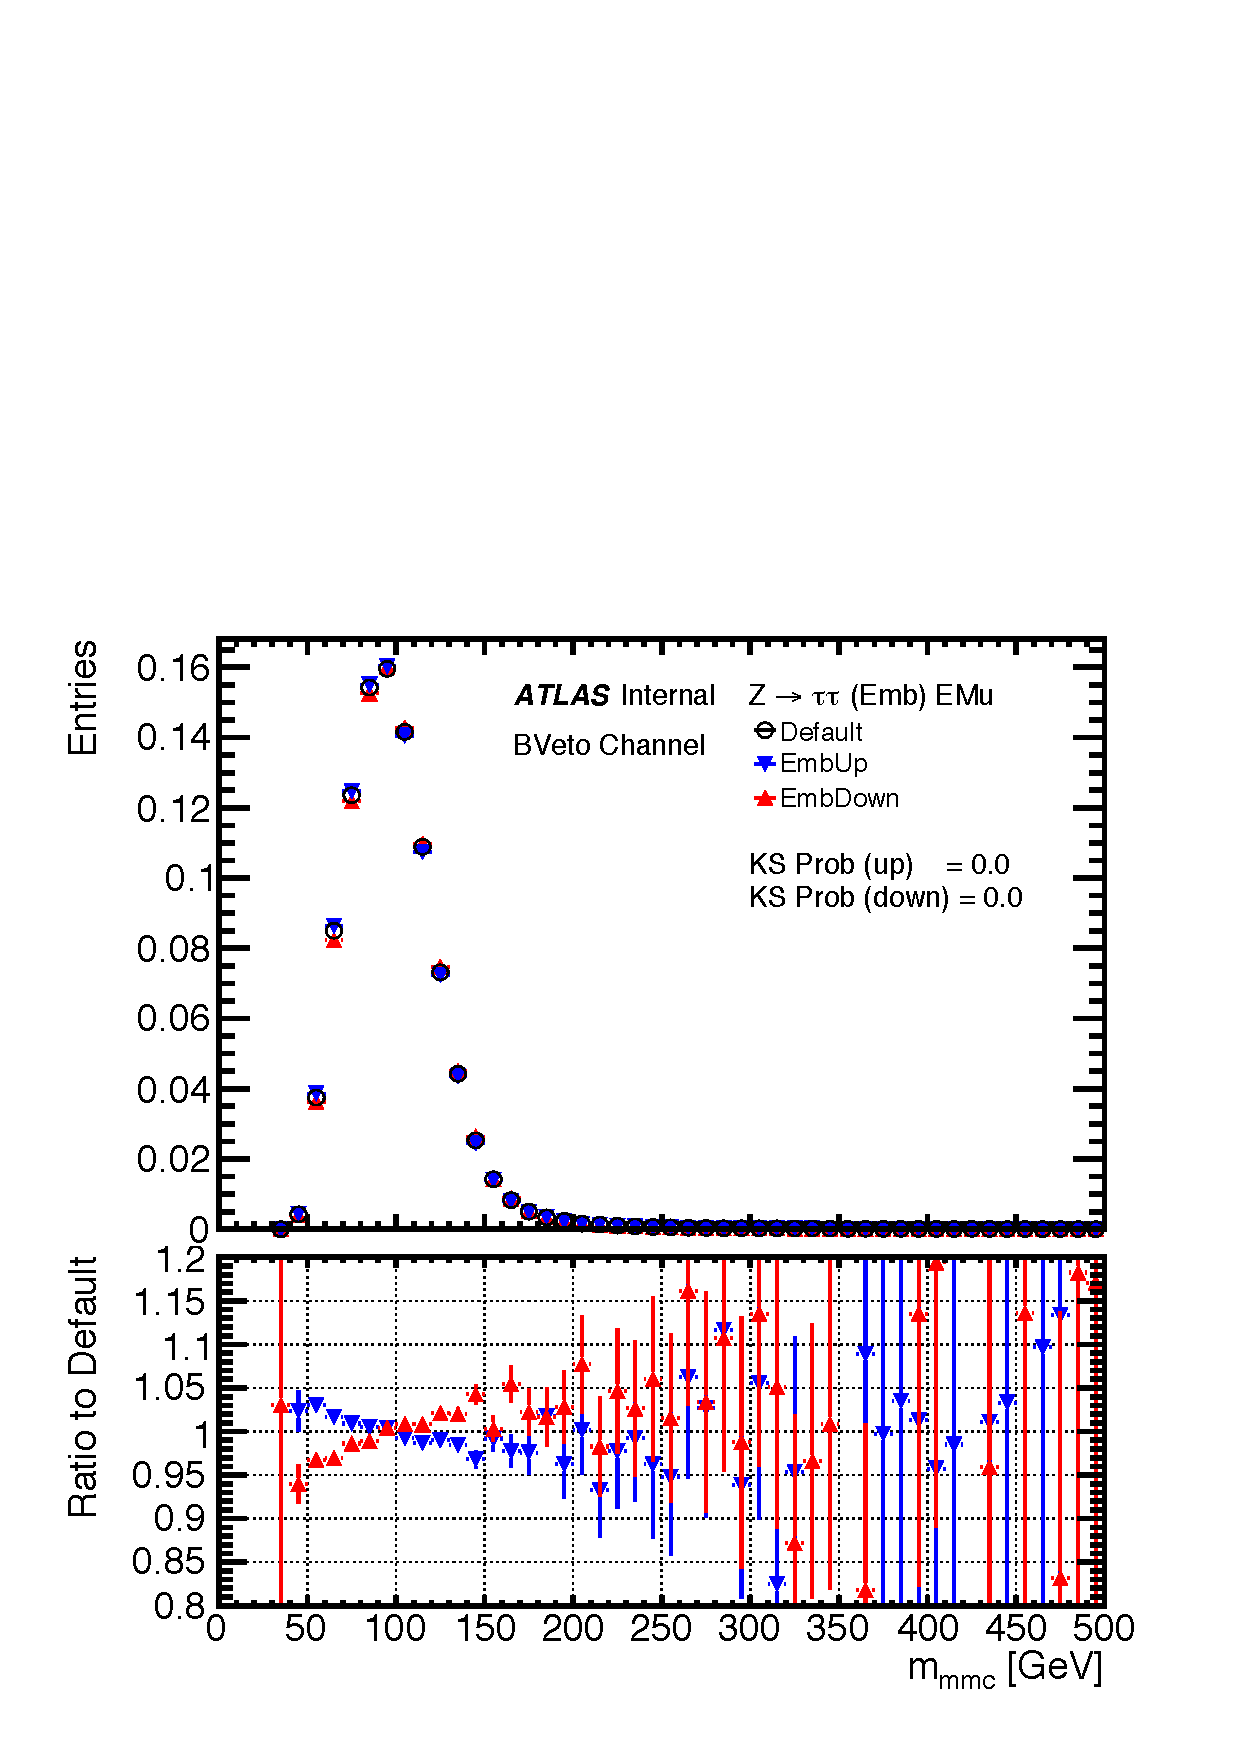
\includegraphics[width=0.45\textwidth]{figure/distributions/NP_Shape_EmbMFS_BVeto_mmc.pdf}
%	}
%	
%        \subfigure[]{%
%            \label{fig:mmc}
%            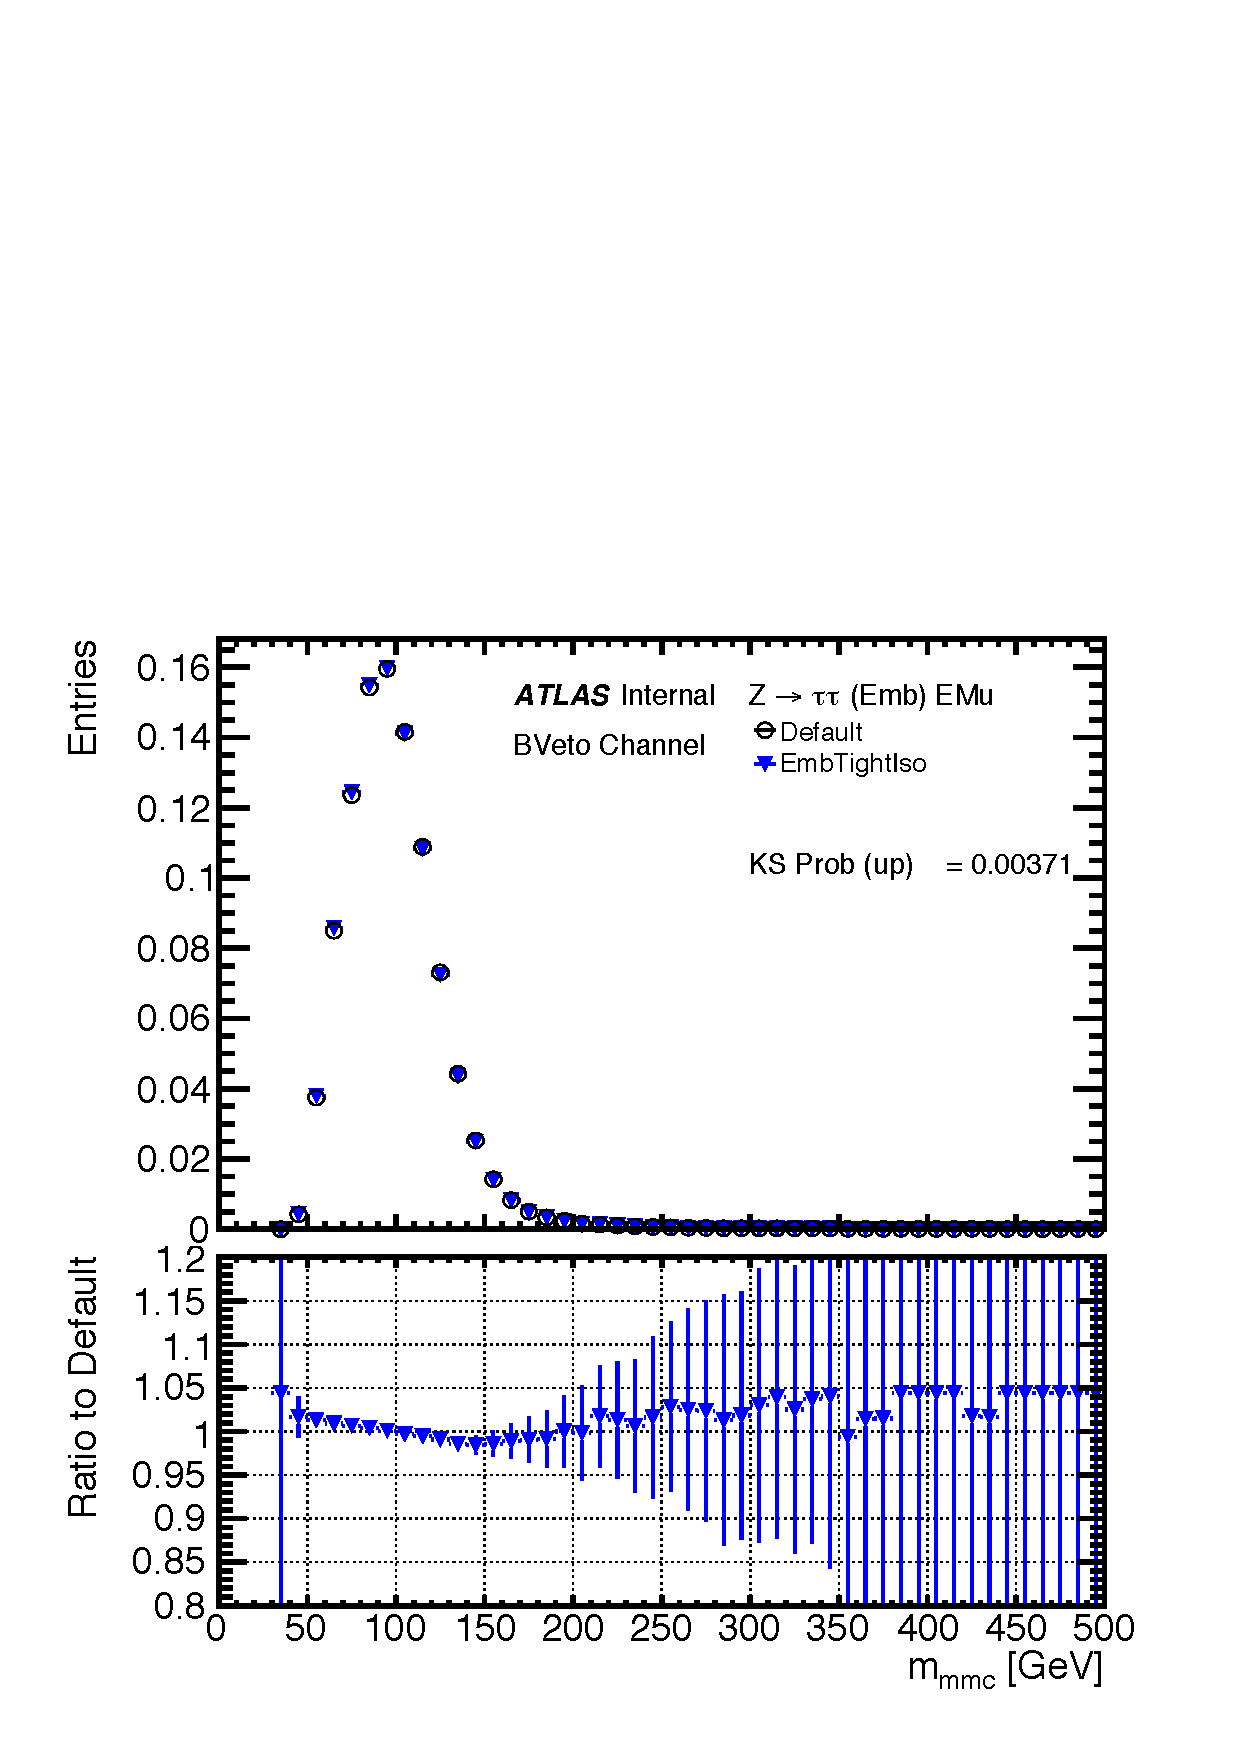
\includegraphics[width=0.45\textwidth]{figure/distributions/NP_Shape_EmbIso_BVeto_mmc.pdf}
%	}
%
%    \end{center}
%    \caption{Effect on the \mmc distribution of the embedding sample due to (a) the EMB\_MFS and (b) embedding isolation systematics. The plots are made after the full b-veto category selection.}
%   \label{fig:embeddingShapeNPs}
%\end{figure}

In the sample of  \Zmumu candidates used for the embedding,  only a loose requirement on the  muon track isolation is applied.
A different  muon isolation requirement may affect the selected sample by modifying the topology of the event, 
% since the requirement is indirectly acting also on the muon \PT, 
changing the contamination with other processes or the activity in the calorimeter. 
To estimate  the importance of these effects in the
embedded sample, the muon isolation criteria used in  the original \Zmumu sample are tightened,
while an even 
%to $\ptcone 40/ \PT<0.06$ 
%and $\etcone 20/ \PT<0.04$, rather than the nominal selection of only $\ptcone 20/ \PT<0.2 $. 
looser selection would have a rather small impact due to  isolation requirements at the trigger level.
The resulting uncertainty, referred to as "EMB\_ISO", affects both the event yield and the shape of 
the \mmc mass distribution in the embedded sample, as shown in Figure~\ref{fig:EMBMFS}. 

Finally, because the normalization of the embedded sample is determined from the simulated ALPGEN sample, 
the uncertainties related to the cross section and to luminosity are assigned. In addition
all detector-related systematic uncertainties relevant to the decay products of the simulated $\tau$ lepton 
decay are propagated to the embedded sample.
 
%\begin{figure}[tp]
%	\begin{center}
%	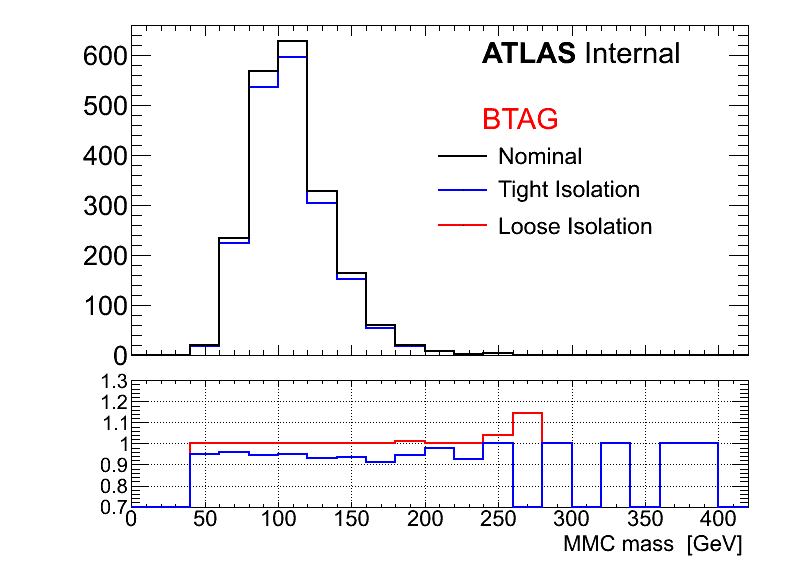
\includegraphics[width=0.49\textwidth]{figure/systematics/emb_sys_BtagFull_Iso.png}
%	\end{center}
%	\caption{embedding Isolation systematic uncertainty impact $\mmc$.}
%	\label{fig:EMBISO}
%\end{figure}

\subsection{QCD Multi-Jet Systematic Uncertainties}\label{sec:qcdsys}
\begin{table} [!tp]
	\begin{center}
	\begin{tabular}{l  c c c }
%%%%%%%%%%%%%%%%%%%%%%%%%%%%%%%%%%%%%%%%%%%%%%%%%%%%%%
\hline 
\hline
Selection  		&  \rqcd  			&  $\rqcd^{AB}$  		&  $R_{QCD}^{iso}$ \\ 
\hline
common selection 		&   1.929 $\pm$     0.004	&	2.12 $\pm$ 0.17		&	2.22 $\pm$ 0.16	\\
No b-tagged jets		&  1.965   $\pm$   0.005    	& 2.10   $\pm$	0.16 		&	2.22 $\pm$ 0.16	\\
Exactly one b-tagged jet	&  1.78    $\pm$   0.02 	& 1.9   $\pm$	0.9 		&	2.0  $\pm$ 0.8	\\
\hline
\hline
%%%%%%%%%%%%%%%%%%%%%%%%%%%%%%%%%%%%%%%%%%%%%%%%%%%%%%
	\end{tabular}
	  \caption{Comparison between \rqcd, $\rqcd^{AB}$ and $R_{QCD}^{iso}$ after the common selection stage and after requiring
	or vetoing the presence of b-tagged jets. Only the statistical uncertainty is reported here.
	The value of $\rqcd^{iso}$ is reported for for the lepton isolation threshold which is twice the nominal value,
	while  for  $\rqcd^{AB}$ and \rqcd the nominal values are reported. }
	\label{table:MCsub}
	\end{center}
\end{table}

The QCD multi-jet background is estimated via the ABCD method, as
described in Section~\ref{sec:qcd}. This technique relies strongly on
the assumption that the lepton isolation variables are uncorrelated to the relative
charge of the two leptons. Systematic uncertainties
are assigned to take into account possible deviations from this assumption.
First the correlation between the ratio  \rqcd and the lepton isolation criteria is considered,
then the result is compared with an auxiliary measurement. 

Figure~\ref{fig:os_ss_ratio} shows the \rqcd factor, i.e. the ratio between the QCD 
yields in data samples C and D, as a function of a sliding lepton isolation threshold relative to the 
nominal analysis selection (red points).
%correlation is clearly visible. 
As described previously, the expected contamination of  non-QCD background processes is subtracted from the data in samples C and D.
To estimate the uncertainty on the value of \rqcd  an additional transfer factor is defined: $R_{QCD}^{iso}  = N_{\hat{A}} / N_{\hat{B}}$,
where  $\hat{A}$ and $\hat{B}$  are semi-isolated OS and SS samples defined by requiring the lepton isolation to be  larger 
than the nominal one, 
but smaller than a given sliding threshold value (defined by the $X$-axis of the plot). Also here the non-QCD contributions are subtracted from the data yields.
%$R_{QCD}^{iso}$ is an attempt to calculate a best estimate for the QCD transfer factor between isolated samples,
%which is in definitive the goal of the ABCD method. 
The semi-isolated samples $\hat{A}$ and $\hat{B}$ are chosen  
given the high contamination with non-QCD background processes and with possible signal in data samples A and B. 
Figure~\ref{fig:os_ss_ratio} shows $R_{QCD}^{iso}$ as a function of the relative lepton isolation threshold (black points).
The difference between \rqcd and $R_{QCD}^{iso} $ in the vicinity of the nominal isolation threshold
is then assigned as a systematic uncertainty on \rqcd. For the lepton isolation threshold which is 
twice the nominal value, a systematic uncertainty of 15\% is found.
The result shown  in Figure~\ref{fig:os_ss_ratio} are obtained  after common selection. Similar results after the full analysis selection
in the two event categories are shown in Appendix~\ref{appendix:qcd_additional}.

%for the definition of lepton isolations used in this analysis, the ratio is calculated in samples where the isolation requirements are reversed. Due to a high contamination of signal and non-QCD backgrounds, "semi-isolated" OS and SS samples are additionally defined, where the lepton isolation is larger than the standard requirement, but less than a sliding cut. These samples are labelled $\hat{A}$ and $\hat{B}$  for the semi-isolated OS and SS samples, respectively, and hence we can define $R_{QCD}^{iso}  = \hat{A} / \hat{B}$. The difference between \rqcd and $R_{QCD}^{iso} $ in the vicinity of our standard cut value is then assigned as a systematic uncertainty on \rqcd. Using the point where the cuts on the lepton isolation are twice their standard values, i.e.. the $x=100\%$ point on the graph, a systematic uncertainty of 15\% is found.

%An additional method considers calculating $\rqcd^{AB}$ as the ratio between the estimated QCD contributions in sample A and B.
%These samples, however, suffers of large contribution of non-QCD background and possible signal contamination, 
%this method is then only used as a cross check. Table~\ref{table:MCsub} shows a comparison between \rqcd and  $\rqcd^{AB}$
%for the two category at an early stage of the cut-flow where signal contamination is negligible, agreement is seen within statistical uncertainties.

As a test of the result described above an additional measurement is performed.
The $\rqcd^{AB}$ is calculated as the ratio between the estimated QCD multi-jet contributions in samples A 
and B instead of C and D. The non-QCD contributions are subtracted from data. Due to the large contribution of this non-QCD background, 
along with small numbers of observed events and possible signal contamination, this measurement is only used for cross check. Table~\ref{table:MCsub} shows 
a comparison between \rqcd, $\rqcd^{iso}$ and $\rqcd^{AB}$ after the common selection stage and after requiring
or vetoing the presence of b-tagged jets,  at these selection stages the signal contamination is negligible. 
Good agreement is seen between the results of these methods. 

%\footnote{This effect is maybe due to the use of a \PT dependent isolation variable that effects the quark-gluon fraction.}.
%Expectation for non-QCD backgrounds are subtracted as usual. 
%This effect however doesn't tell anything on the uncertainty of our
%measure of \rqcd, we want to measure instead what is the discrepancy (for each
%chosen isolation cut value) between \rqcd and the same factor calculated 
%flipping isolation requirements, i.e. using the isolated samples A and B, we call this factor $R_{QCD}^{iso}$. 
%Due to the high contamination of non-QCD backgrounds and signal in these samples we then define:
%OS and SS isolated samples $\hat{A}$ and $\hat{B}$ in which the leptons isolation
%should be greater than the standard value but less of predefined quantity on the x axis 
%of the graph (black curve). In definitive we have $R_{QCD}^{iso}  = \hat{A} / \hat{B}$.
%We then assign as a systematics uncertainty the difference between the two curves (red and black) in the vicinity of our
%standard cut value (we use the point where the cut value is doubled, 100\% in the graph because 
%of statistical fluctuation), our estimate of the systematics uncertainty on \rqcd is then 15\%.
%The plot in Figure~\ref{fig:os_ss_ratio} is made at common selection level, similar plots using the full selection
%for the two categories are in Appendix~\ref{appendix:qcd_additional}.

%An additional method used as a crosscheck relies on the definition of "real-$\rqcd$" as the pure ratio between sample A and B (non-QCD background
%estimate is subtracted from data in each samples), this would be the exact factor 
%that allows you to extrapolate yield from sample B to SR, however it suffer of contamination by non-QCD backgrounds
%and lack of statistics.
%Table~\ref{table:MCsub} shows comparison between \rqcd and real-\rqcd
%for the two category at an early stage of the cut-flow where signal contamination is negligible.
%Discrepancies are within statistical uncertainty and underline that an assignment of a  15\%
%uncertainty to the \rqcd factor is conservative.


The shape of the \mmc mass distribution differs between the OS and SS in 
anti-isolated samples (C and D) as shown in Figure~\ref{fig:qcd_shape_unc}.
The size of this effect is within the above \rqcd uncertainty for the  relevant mass range of the QCD multi-jet background (QCD multi-jet background
contribution is negligible for $\mmc  > 150$ GeV) and hence no correction factor is applied to the mass shape of sample B. 
It is assumed, however, that there could be the same 
shape difference in the isolated samples and thus a shape uncertainty is  assigned to the mass distribution in 
sample B to account for this  deviation. Further 
shape uncertainties due to non-QCD background subtraction are found to be negligible. The uncertainty due to the use of an isolation 
requirement at the trigger level is discussed in Appendix~\ref{appendix:qcd} and is found to be negligible.



\begin{figure}[ht]
	\begin{center}
	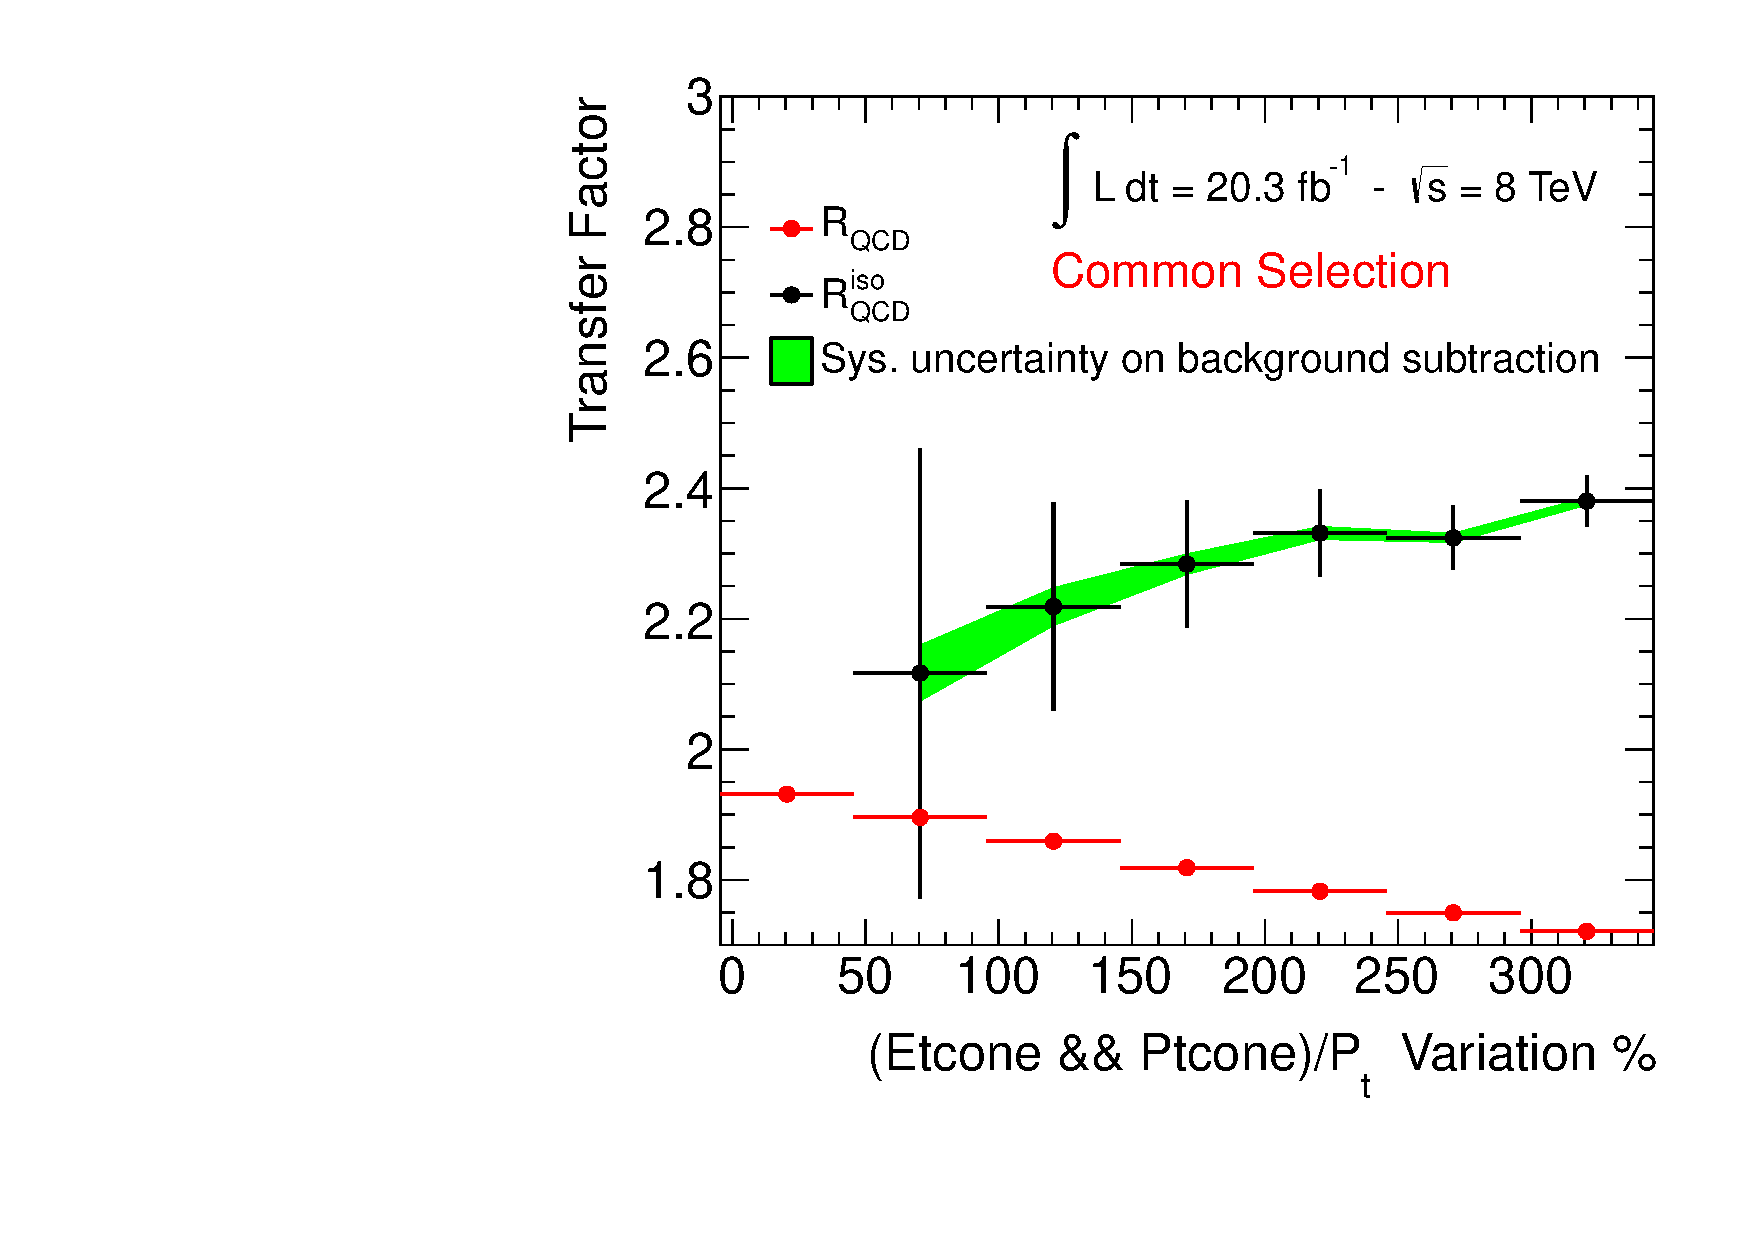
\includegraphics[width=0.60\textwidth]{figure/systematics/QCD_presel_SYS.pdf}
	\end{center}
	\caption{Transfer factors \rqcd and $R_{QCD}^{iso}$  (see text) as a function of the sliding lepton isolation 
	thresholds. The thresholds are varied in percentages relative to the nominal lepton isolation threshold (value of zero on the plot).
	The common selection are applied.
	%As an example the point at 100\% in the plot corresponds
	%to $\rqcd$ evaluated by increasing the isolation requirement by 100\% respect to the standard cut value.
%	The red points show the anti-isolated scale factor $\rqcd$, i.e. the ratio between samples C and D.
%	 The black points show the isolated scale factor, which is defined as the ratio between sample $\hat{A}$ and $\hat{B}$, 
%	 where the leptons have isolation values larger than the nominal value but smaller
%	 than the sliding cut on X axis.
%	 taking the same example point at 100\%, than the double of the standard cut value.
	 }
	\label{fig:os_ss_ratio}
\end{figure}

\begin{figure}[h]
	\begin{center}
	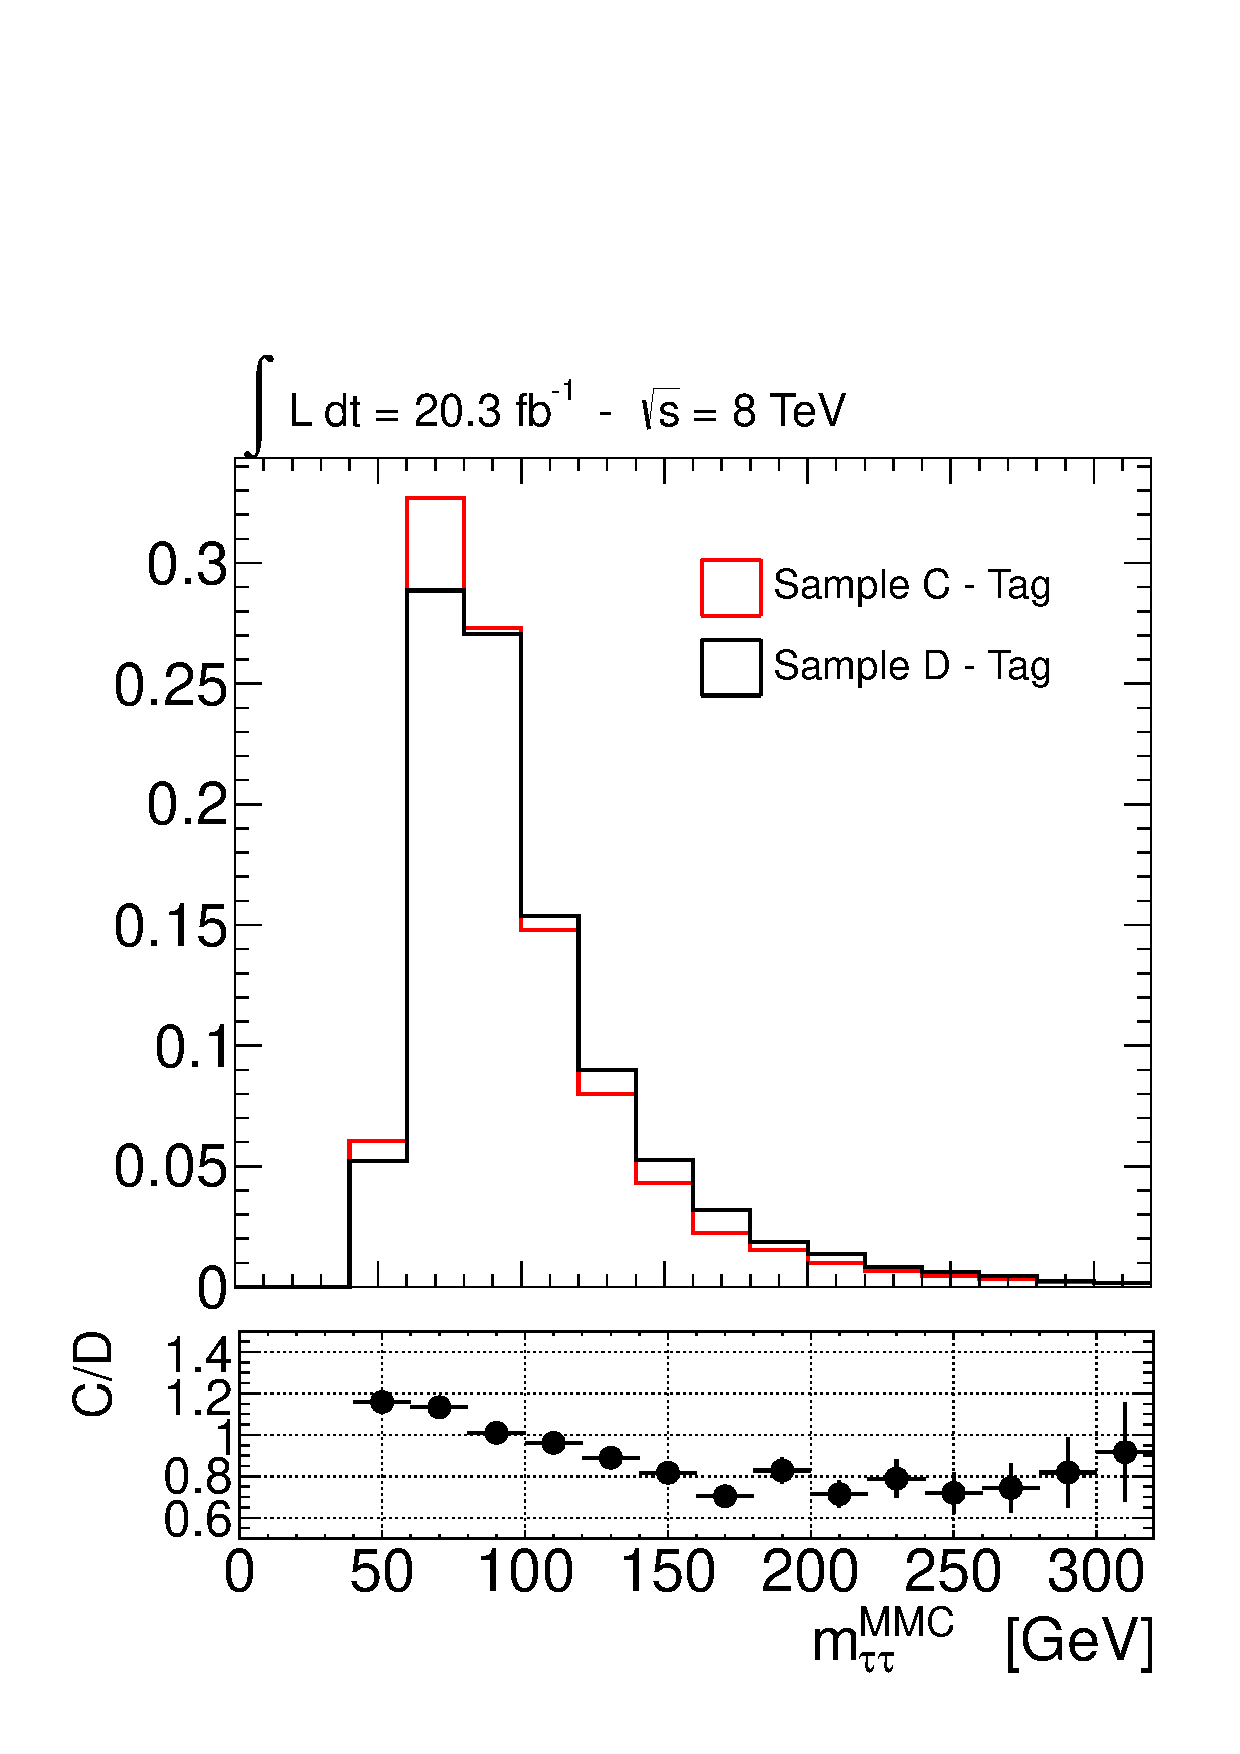
\includegraphics[width=0.47\textwidth]{figure/systematics/qcd_shape_tag.pdf}
	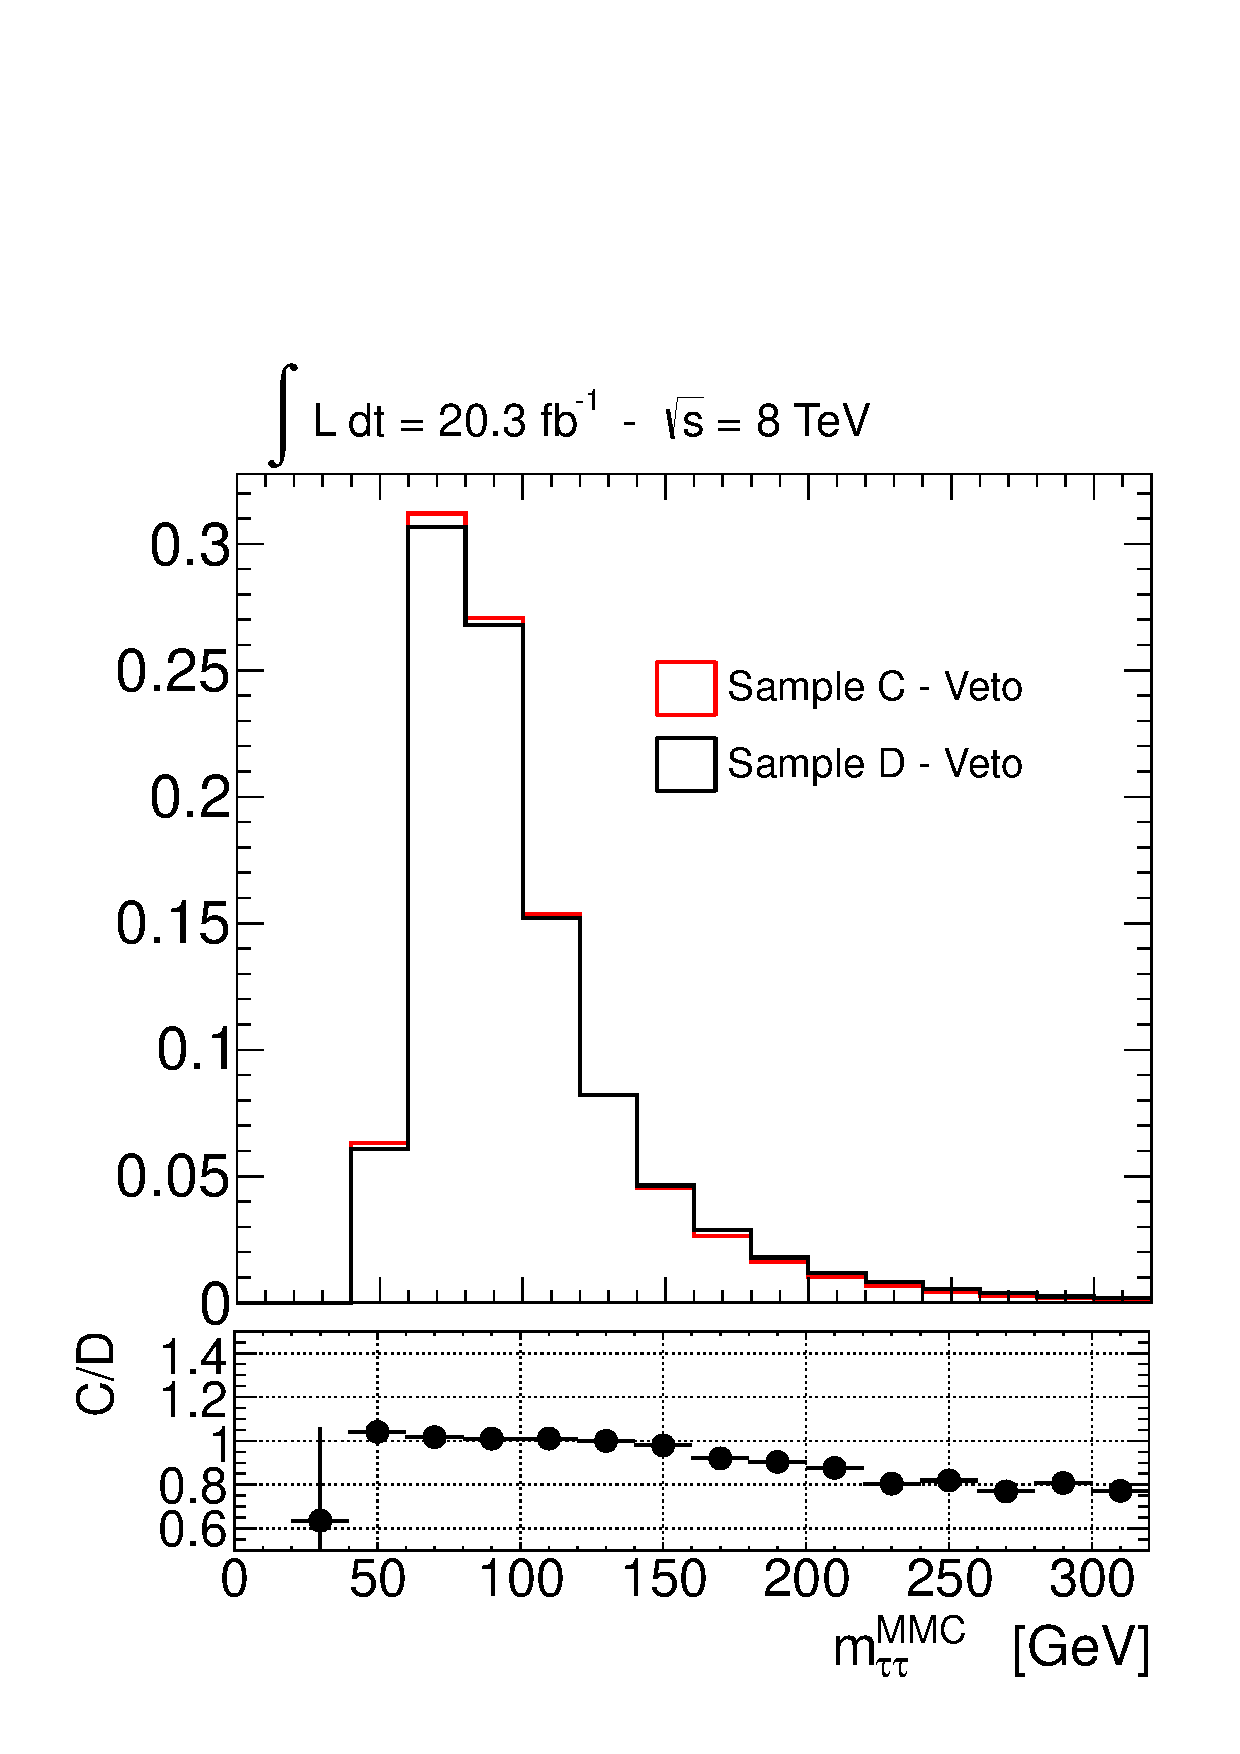
\includegraphics[width=0.47\textwidth]{figure/systematics/qcd_shape_veto.pdf}
	\end{center}
	\caption{Differences in the shape of the invariant \mmc mass distribution in data samples  C and D shown 
	separately for the b-taged  and b-vetoed event categories. The data samples C and D are normalised to the same 
	number of events.}
	\label{fig:qcd_shape_unc}
\end{figure}






